
\section{Convolutional autoencoder}
A convolutional autoencoder(CAE) consists of two parts, namely the encoding part and decoding part. While the decoded output may not be the same as the input, the goal is to restore the input as much as possible. A sample CAE is shown in the graph. There is only a convolution layer in the encoder part and a de-convolution layer in the decoder part for this example.

\begin{figure}[htbp]
\centering{
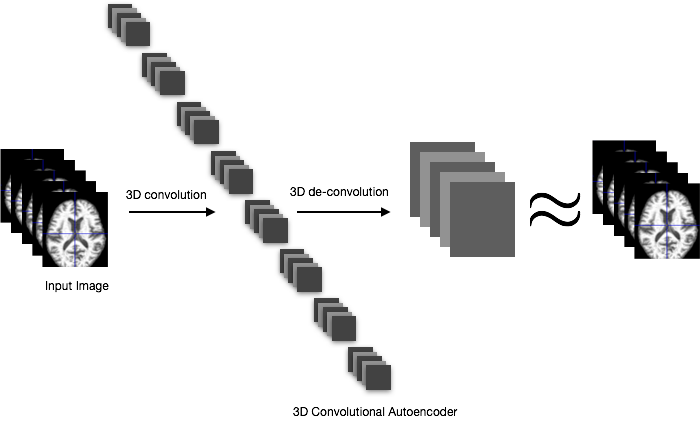
\includegraphics[width=.5\textwidth]{CAE.png}}
\caption{Convolutional autoencoder}
\end{figure}


\subsection{Encoder}
We can put convolution layers and pooling layers in the encoding part as the normal CNN to get the encoded output. For this specific CAE here, we use a convolution layer only.
Suppose the input data is denoted as $X$, the kernel for the convolution layer is $K^1$. We can obtain the encoded output $Y$ by convolution as
\begin{align}
    K^1 * X  = Y.
\end{align}
%Then with the backpropagation, the input and the parameters can be updated as 
%\begin{align}
%   dY * (K^1)^T = dX,   \\
%   dY * X      = dK^1 .
%\end{align}
If we rewrite the convolution in the form of matrix multiplication, it becomes
\begin{align}
   Y = K^1 * X = T \cdot X.
\end{align}
For the purpose of illustration, we take $K^1 \in \mathbb{R}^4$, $X \in \mathbb{R}^8$ with the stride to be 2. Then we have $Y \in \mathbb{R}^5$ and $T \in \mathbb{R}^{5*8}$.

Suppose $K^1=(k_1, k_2, k_3, k_4)$ and $X=(x_1, x_2, ..., x_8)$. The corresponding coefficient matrix $T$ can be represented as 
\begin{align}
   T = P \cdot \tilde{T} &= 
%  \begin{bmatrix}
%    (1-2r)  & -r      & 0       & \cdots  & 0  \\
%    -r      & (1-2r)  & -r      & \ddots  & \vdots   \\
%     0      &  \ddots & \ddots  & \ddots  & 0  \\
%    \vdots  &         & -r      & (1-2r)  & -r  \\
%     0      & \cdots  & 0       & -r      & (1-2r)
%  \end{bmatrix}
\left(
  \begin{array}{ccccccccc}
     1 & 0 & 0 & 0 & 0 & 0 & 0 & 0 & 0 \\
     0 & 0 & 1 & 0 & 0 & 0 & 0 & 0 & 0 \\
     0 & 0 & 0 & 0 & 1 & 0 & 0 & 0 & 0 \\
     0 & 0 & 0 & 0 & 0 & 0 & 1 & 0 & 0 \\
     0 & 0 & 0 & 0 & 0 & 0 & 0 & 0 & 1 \\
  \end{array}
\right)_{5*9}
\left(
  \begin{array}{cccccccc}
     k_3 & k_4 & 0 & 0 & 0 & 0 & 0 & 0  \\
     k_2 & k_3 & k_4 & 0 & 0 & 0 & 0 &  0 \\
     k_1 & k_2 & k_3 & k_4 & 0 & 0 & 0 & 0  \\
     0 & k_1 & k_2 & k_3 & k_4 & 0 & 0 & 0  \\
     0 & 0 & k_1 & k_2 & k_3 & k_4 & 0 & 0  \\
     0 & 0 & 0 & k_1 & k_2 & k_3 & k_4 & 0  \\
     0 & 0 & 0 & 0 & k_1 & k_2 & k_3 & k_4  \\
     0 & 0 & 0 & 0 & 0 & k_1 & k_2 & k_3   \\
     0 & 0 & 0 & 0 & 0 & 0 & k_1 & k_2  \\
  \end{array}
\right)_{9*8}\\ \notag 
&= 
\left(
  \begin{array}{cccccccc}
     k_3 & k_4 & 0 & 0 & 0 & 0 & 0 & 0  \\
     k_1 & k_2 & k_3 & k_4 & 0 & 0 & 0 &  0 \\
     0 & 0 & k_1 & k_2 & k_3 & k_4 & 0 &  0  \\
     0 & 0 & 0 &0 & k_1 & k_2 & k_3 & k_4   \\
     0 & 0 & 0 & 0 & 0 & 0 & k_1 & k_2    \\
  \end{array}
\right)_{5*8}.
\end{align}
Here $P$ denote the operation of stride being 2 and $\tilde{T}$ is the standard convolution operation.

The procedure can be illustrated as below.
\begin{figure}[htbp]
\centering{
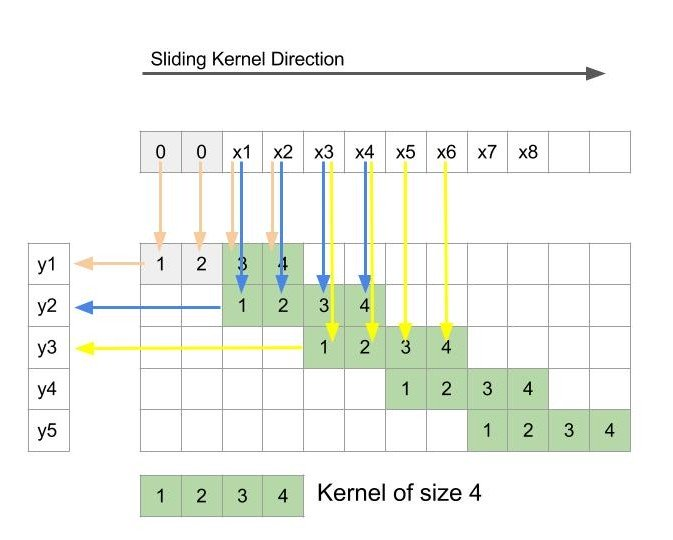
\includegraphics[width=.6\textwidth]{conv.jpeg}}
\caption{Depiction of usual convolution process with 1-d input}
\end{figure}


\subsection{Decoder}
We can put unpooling layers and deconvolution layers in the decoding part to get the decoded output. For this specific CAE here, we use a deconvolution layer only.
Suppose the encoded data from the encoder is denoted as $Y$ and the restored output as $\tilde{X}$. In TensorFlow, $\tilde{X}$ is obtained from $Y$ with the function tf.nn.conv3d$\_$transpose. 

Here is what tf.nn.conv3d$\_$transpose does.
It construct another CNN with a convolution layer only, which takes $Y$ as the output and $\tilde{X}$ as the input. Then  the input is updated with the backpropagation by the function gen$\_$nn$\_$ops.conv3d$\_$backprop$\_$input$\_$v2. %This function does the following operation.

If we rewrite the deconvolution in the form of matrix multiplication, it becomes
\begin{align}
   \tilde{X} = K^2 * Y = T^T \cdot Y.
\end{align}

%Suppose $Y$ can be obtained by convolution as
%\begin{align}
%    K^2 * \tilde{X}  = Y.
%\end{align}
%Then with the backpropagation, the input and the parameters can be updated as
%\begin{align}
%   dY *(K^2)^T  = d\tilde{X},   \\
%   dY * \tilde{X}      = dK^2.
%\end{align}
%After $\tilde{X}$ is updated, the $L^2$ loss function is used to compute the difference between $X$ and $\tilde{X}$. 

With the same notation as above, the corresponding coefficient matrix $T^T$ can be represented as 
\begin{align}
   T^T = \tilde{T}^T\cdot  P^T &= 
%  \begin{bmatrix}
%    (1-2r)  & -r      & 0       & \cdots  & 0  \\
%    -r      & (1-2r)  & -r      & \ddots  & \vdots   \\
%     0      &  \ddots & \ddots  & \ddots  & 0  \\
%    \vdots  &         & -r      & (1-2r)  & -r  \\
%     0      & \cdots  & 0       & -r      & (1-2r)
%  \end{bmatrix}
\left(
  \begin{array}{ccccccccc}
     k_3 & k_2 & k_1 & 0 & 0 & 0 & 0 & 0  & 0\\
     k_4 & k_3 & k_2 & k_1 & 0 & 0 & 0 &  0 & 0\\
     0 & k_4 & k_3 & k_2 & k_1 & 0 & 0 & 0 & 0\\
     0 & 0 & k_4 & k_3 & k_2 & k_1 & 0 & 0  & 0\\
     0 & 0 & 0 & k_4 & k_3 & k_2 & k_1 & 0  & 0\\
     0 & 0 & 0 & 0 & k_4 & k_3 & k_2 & k_1  & 0\\
     0 & 0 & 0 & 0 & 0 & k_4 & k_3 & k_2 & k_1  \\
     0 & 0 & 0 & 0 & 0 & 0  & k_4 & k_3 & k_2   \\
  \end{array}
\right)_{8*9}
\left(
  \begin{array}{ccccc}
     1 & 0 & 0 & 0 & 0  \\
     0 & 0 & 0 & 0 & 0  \\
     0 & 1 & 0 & 0 & 0  \\
     0 & 0 & 0 & 0 & 0  \\
     0 & 0 & 1 & 0 & 0  \\
     0 & 0 & 0 & 0 & 0  \\
     0 & 0 & 0 & 1 & 0  \\
     0 & 0 & 0 & 0 & 0  \\
     0 & 0 & 0 & 0 & 1  \\
  \end{array}
\right)_{9*5}
\\ \notag 
&= 
\left(
  \begin{array}{ccccc}
     k_3 & k_1 & 0 & 0 & 0   \\
     k_4 & k_2 & 0 & 0 & 0   \\
     0 & k_3 & k_1 & 0 & 0  \\     
     0 & k_4 & k_2 & 0 & 0  \\
     0 & 0 & k_3 & k_1 & 0  \\
     0 & 0 & k_4 & k_2 & 0  \\
     0 & 0 & 0 & k_3 & k_1  \\
     0 & 0 & 0 & k_4 & k_2  \\
  \end{array}
\right)_{8*5}.
\end{align}
Here $P^T$ denote the operation of padding(adding zeros) and $\tilde{T}$ is the standard deconvolution operation.

The procedure can be illustrated as below.
\begin{figure}[htbp]
\centering{
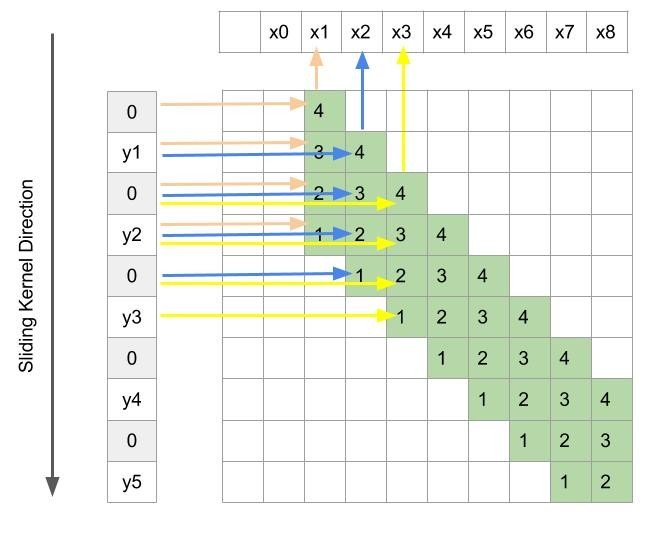
\includegraphics[width=.6\textwidth]{deconv.jpeg}}
\caption{Deconvolution}
\end{figure}

\section{Denoising by Convolutional Autoencoder}

\paragraph{Autoencoder}
    \begin{itemize}
        \item An Autoencoder is a neural network that is trained to attempt to copy its input to its output.
        \item The network consists of two parts
            \begin{itemize}
                \item An encoder function
                    \begin{equation*}
                        h=f(x).
                    \end{equation*}
                \item A decoder function that produce a reconstruct
                    \begin{equation*}
                        y=g(h).
                    \end{equation*}
            \end{itemize}
        \item The goal for training the network is to minimize the difference between the output $y$ and  the input $x$
            $$
                \min \|g(f(x))-x\|_{\ell^2}.
            $$
    \end{itemize}


A convolutional autoencoder is an autoencoder consists of convolutional layers.  
    
A simple CAE with one hidden layer 
\begin{itemize}
\item Convolution
    $$h=f(x)=K\circledast x+\operatorname{diag}(b)I.$$

\item De-convolution

    Inverse operation of the convolution to restore the input
        $$y=g(h)=\hat{K}\circledast h+\operatorname{diag}(\hat b)I.$$


\item We train the model 
    $$y=g(f(x))$$
   to solve the following minimization problem 
        $$\min\|y-x\|_{\ell^2}$$
\item Then we use $f$ as the encoder, and $g$ as the decoder.

\end{itemize}

    \begin{center}
        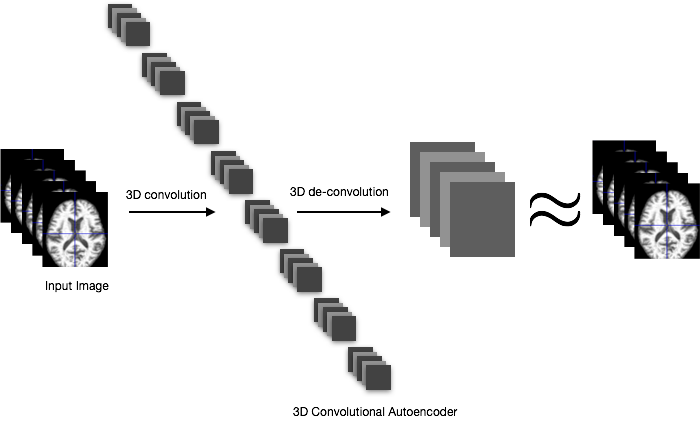
\includegraphics[width=0.8\textwidth]{CAE}
    \end{center}

\paragraph{MNIST with noise}
    \begin{itemize}
        \item We add Gaussian noise to MNIST dataset
            \begin{equation*}
                x_{ij} \leftarrow x_{ij}+\eta z,
            \end{equation*}
            where $z$ is the Gaussian random variable given by 
            \begin{equation*}
                P(z)= \frac{1}{\sigma\sqrt{2\pi}}e^{-\frac{(z-\mu)^2}{2\sigma^2}}
            \end{equation*}
         \item Then construct a CAE model such that given an image with noise, it will output the denoised image.

             \begin{center}
                 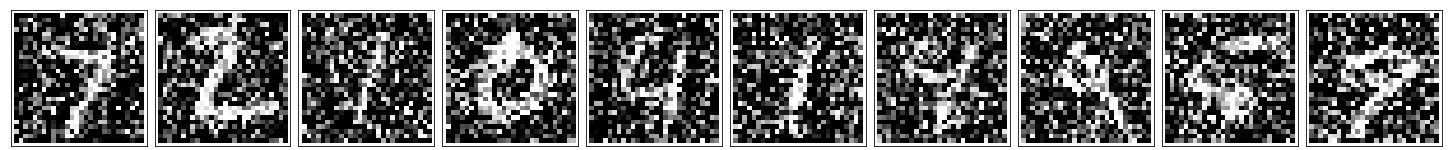
\includegraphics[width=0.8\textwidth]{noise}
             \end{center}
    \end{itemize}
    \begin{center}
        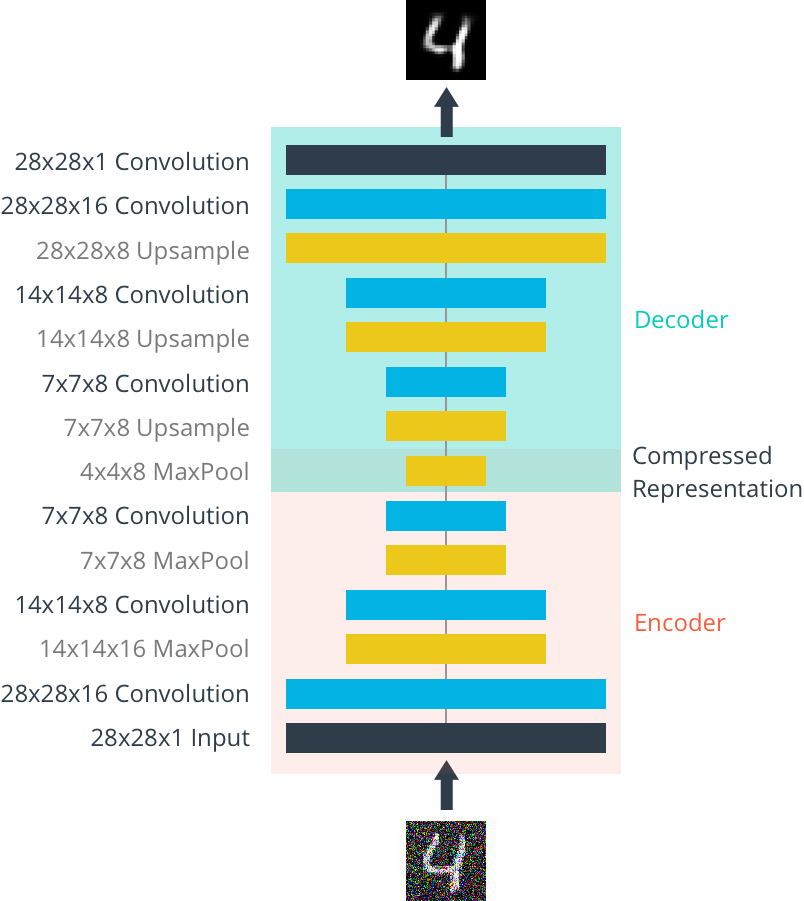
\includegraphics[height=0.8\textheight]{denoise}
    \end{center}


    \paragraph{Encoder:}
    \begin{itemize}
    \footnotesize
    \item  First convolutional layer:
    \begin{equation*}
        f^0 = \theta^0(x) \in \mathbb{R}^{16\times 28\times 28},
    \end{equation*}
    with
    \begin{equation*}
        \theta^0(x) = K^0 \circledast x + {\rm{diag}(b^0) }\cdot \bm{1} \quad, \quad K^0 \in R^{16 \times 1 \times 3 \times 3}, \quad b^0 \in \mathbb R^{16}
    \end{equation*}
    \item  Second convolutional layer:
    \begin{equation*}
        f^1 = \theta^1(r^1(\sigma^1 (f^0)))\in \mathbb{R}^{8\times 14\times 14},
    \end{equation*}
            where $\sigma^1: \mathbb{R}^{16\times 28\times 28}\mapsto \mathbb{R}^{16\times 28\times 28}$ is the ReLU activation function; $r^1:\mathbb{R}^{16\times 28\times 28}\mapsto \mathbb{R}^{8\times 14\times 14}$ is the max-pooling function; and 
            \begin{equation*}
                \theta^1(x) = K^1 \circledast x + {\rm{diag}(b^1) }\cdot \bm{1} \quad, \quad K^1 \in \mathbb R^{8 \times 16 \times 3 \times 3}, \quad b^1 \in \mathbb R^{8}.
            \end{equation*}
    \item  Third convolutional layer:
    \begin{equation*}
        f^2 = \theta^2(r^2(\sigma^2 (f^1)))\in \mathbb{R}^{8\times 7\times 7},
    \end{equation*}
            where $\sigma^2: \mathbb{R}^{8\times 14\times 14}\mapsto \mathbb{R}^{8\times 14\times 14}$ is the ReLU activation function; $r^2:\mathbb{R}^{8\times 14\times 14}\mapsto \mathbb{R}^{8\times 7\times 7}$ is the max-pooling function; and 
            \begin{equation*}
                \theta^2(x) = K^2 \circledast x + {\rm{diag}(b^2) }\cdot \bm{1} \quad, \quad K^1 \in \mathbb R^{8 \times 8 \times 3 \times 3}, \quad b^2 \in \mathbb R^{8}.
            \end{equation*}
    \end{itemize}

    \paragraph{Output of encoder:}
        \begin{equation*}
            f = r^3(\sigma^3(f^2))\in \mathbb{R}^{8\times 4\times 4},
        \end{equation*}
            where $\sigma^3: \mathbb{R}^{8\times 7\times 7}\mapsto \mathbb{R}^{8\times 7\times 7}$ is the ReLU activation function; $r^3:\mathbb{R}^{8\times 7\times 7}\mapsto \mathbb{R}^{8\times 4\times 4}$ is the max-pooling function. 

            \begin{center}
                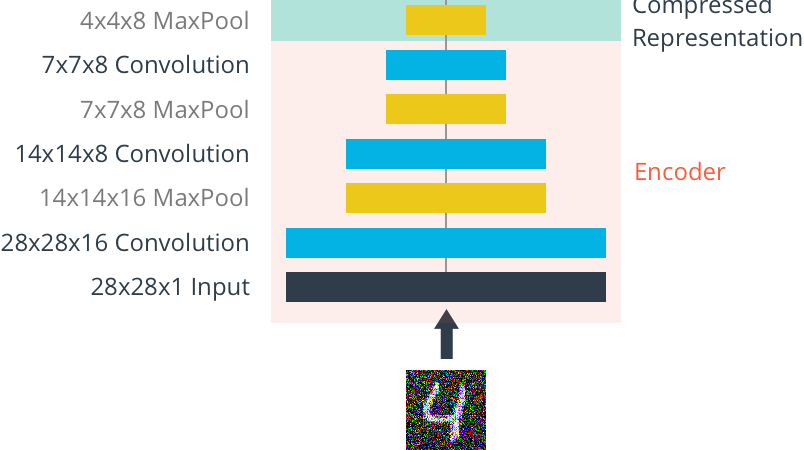
\includegraphics[width=0.5\textwidth]{encoder}
            \end{center}

    \paragraph{Decoder:}
    \begin{itemize}
        \footnotesize
        \item First deconvolutional layer:
            \begin{equation*}
                g^1=\hat\theta^1 (p^1(f))\in \mathbb{R}^{8\times 7\times 7},
            \end{equation*}
            where $p^1: \mathbb{R}^{8\times 4\times 4}\mapsto \mathbb{R}^{8\times 7\times 7}$ is the up-pooling function; and 
            \begin{equation*}
                \hat\theta^1(x) = \hat K^1 \circledast x + {\rm{diag}(\hat b^1) }\cdot \bm{1} \quad, \quad \hat K^1 \in \mathbb R^{8 \times 8 \times 3 \times 3}, \quad \hat b^1 \in \mathbb R^{8}.
            \end{equation*}
        \item Second deconvolutional layer:
            \begin{equation*}
                g^2=\hat\theta^2 (p^2(\hat\sigma^2(g)))\in \mathbb{R}^{8\times 14\times 14},
            \end{equation*}
            where $\hat\sigma^2: \mathbb{R}^{8\times 7\times 7}\mapsto \mathbb{R}^{8\times 7\times 7}$ is the ReLU activation function; 
            $p^2: \mathbb{R}^{8\times 7\times 7}\mapsto \mathbb{R}^{8\times 14\times 14}$ is the up-pooling function; and 
            \begin{equation*}
                \hat\theta^2(x) = \hat K^2 \circledast x + {\rm{diag}(\hat b^2) }\cdot \bm{1} \quad, \quad \hat K^2 \in \mathbb R^{8 \times 8 \times 3 \times 3}, \quad \hat b^2 \in \mathbb R^{8}.
            \end{equation*}
        \item Third deconvolutional layer:
            \begin{equation*}
                g^3=\hat\theta^3(p^3(\hat\sigma^3(g)))\in \mathbb{R}^{16\times 28\times 28},
            \end{equation*}
            where $\hat\sigma^3: \mathbb{R}^{8\times 14\times 14}\mapsto \mathbb{R}^{8\times 14\times 14}$ is the ReLU activation function; 
            $p^3: \mathbb{R}^{8\times 14\times 14}\mapsto \mathbb{R}^{16\times 28\times 28}$ is the up-pooling function; and
            \begin{equation*}
                \hat\theta^3(x) = \hat K^3 \circledast x + {\rm{diag}(\hat b^3) }\cdot \bm{1} \quad, \quad \hat K^3 \in \mathbb R^{16 \times 8 \times 3 \times 3}, \quad \hat b^3 \in \mathbb R^{16}.
            \end{equation*}
    \end{itemize}

\paragraph{Output of decoder:}
        \begin{equation*}
            f = \hat\theta^4 (\hat\sigma^4(f^2))\in \mathbb{R}^{1\times 28\times 28},
        \end{equation*}
            where $\hat\sigma^4: \mathbb{R}^{16\times 28\times 28}\mapsto \mathbb{R}^{16\times 28\times 28}$ is the ReLU activation function;  and
            \begin{equation*}
                \hat\theta^4(x) = \hat K^4 \circledast x + {\rm{diag}(\hat b^4) }\cdot \bm{1} \quad, \quad \hat K^4 \in \mathbb R^{1 \times 16 \times 3 \times 3}, \quad \hat b^4 \in \mathbb R^{1}.
            \end{equation*}

            \begin{center}
                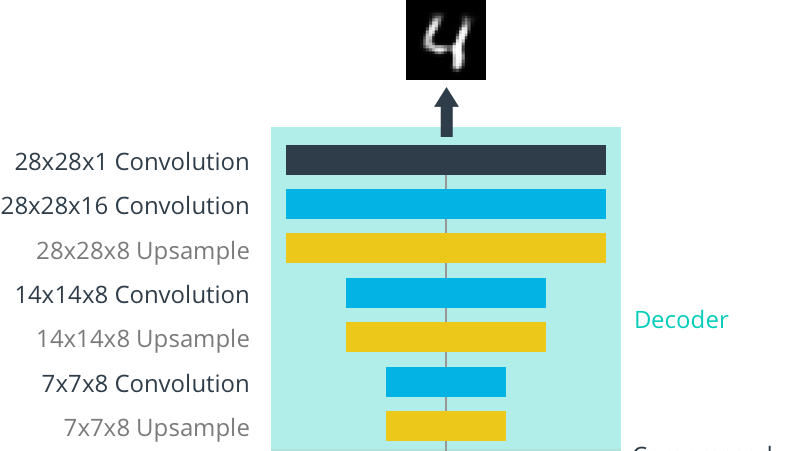
\includegraphics[width=0.5\textwidth]{decoder}
            \end{center}
   After training 100 epochs:

    \begin{center}
        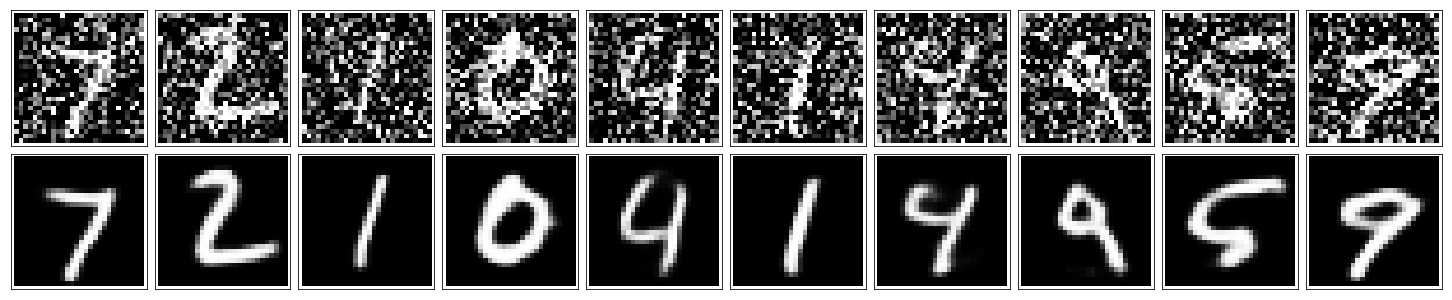
\includegraphics[width=0.8\textwidth]{result}
    \end{center}

\section{Linear encoder, nonlinear encoder and ``enhanced'' encoder}
Deep Neural Network can naturally be viewed as nonlinear encoders. 

Given the data $x\in \mathbb R^d$, we consider the nonlinear encoder
\begin{equation}\label{nonlinear-encoder0}
f(x)=\sigma (W_1x+b_1),  \quad W_1\in \mathbb R^{c\times d}.  
\end{equation}
\begin{equation}\label{nonlinear-encoder}
f(x)=W_2\sigma (W_1x+b_1)+b_2,  \quad W_1\in \mathbb R^{c\times d},
W_2\in\mathbb R^{c\times c}
\end{equation}

We now combine the nonlinear \eqref{nonlinear-encoder} with a linear
encoder to get the following ``enhanced'' encoder:
\begin{equation}\label{enhanced-encoder}
\tilde f(x)=f(x)+\tilde W_1x +\tilde b_1\quad \tilde W_1\in \mathbb R^{c\times d}.
\end{equation}
where
\begin{equation}
\tilde b_1=0 \mbox{ if } b_2=0 \mbox{ or if $f(x)$ is given by \eqref{nonlinear-encoder0}}
\end{equation}

\begin{lemma}
There exists .... such that  
$$
W_2\sigma (W_1x+b_1)+b_2\equiv x
$$
\end{lemma}
\begin{theorem}
Nonlinear encoder recovers linear encoder if $d\le c/2$(?) 
\end{theorem}
Can we make the following statement:
\begin{remark}
  Nonlinear encoder can recover linear encoder in a smaller dimension?
  or coarser grid?
\end{remark}
